\begin{enumerate}[label=\thesubsection.\arabic*.,ref=\thesubsection.\theenumi]
\numberwithin{equation}{enumi} 
\item 
The asymptotic Bode magnitude plot of  minimum phase transfer function
G(s) is show in Fig. \ref{fig:ee18btech11009_bode} .
\begin{figure}[htp]
	\centering
	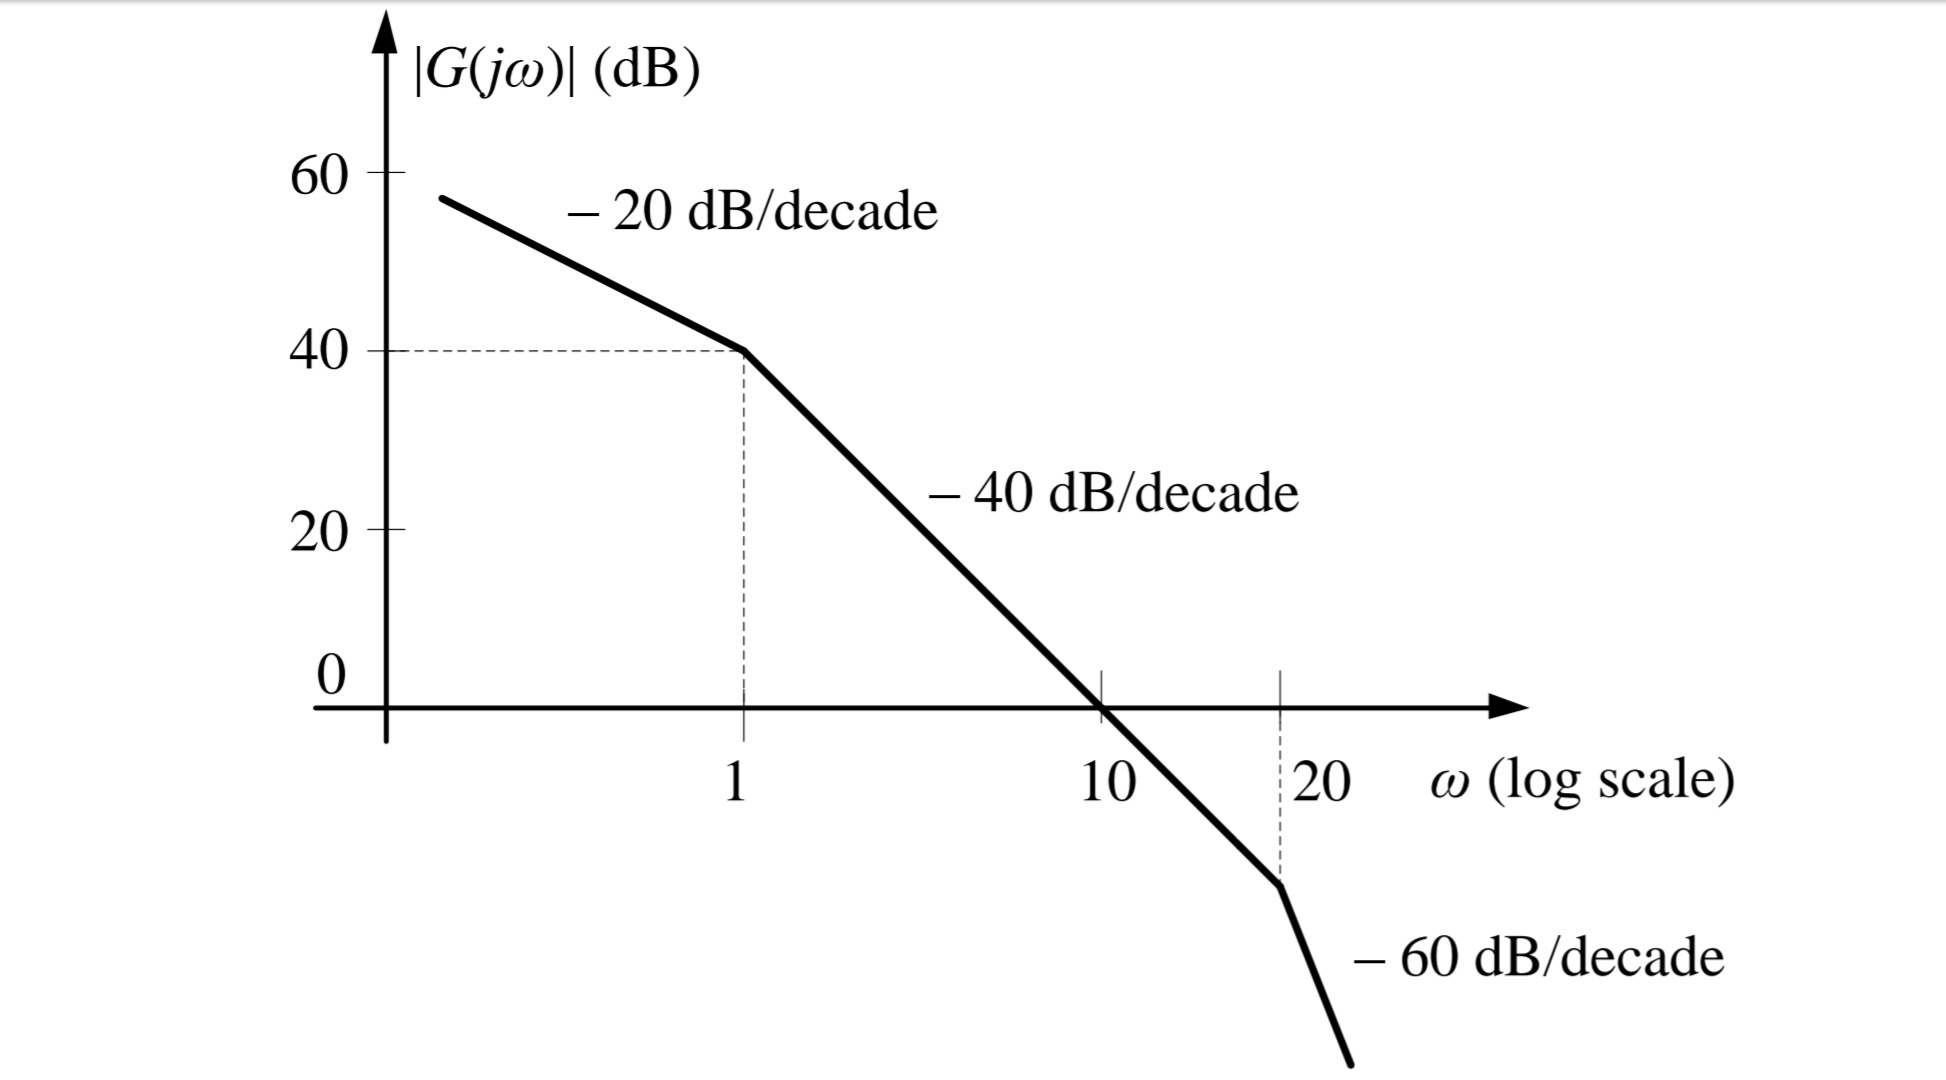
\includegraphics[width=\columnwidth]{./figs/ee18btech11009/pppp.eps}
	\caption{}
	\label{fig:ee18btech11009_bode}
\end{figure} 
%
Express $20\log\abs{G(\j\omega)}$ as a function of $\omega$ using Fig. \ref{fig:ee18btech11009_bode}.
\label{prob:ee18btech11009_bode}
\\
\solution The desired expression (in dB) is
{\footnotesize
\begin{align}
 \abs{G(j\omega)} = 
 \begin{cases}
	60-20(\log(\omega)-\log(0.1)) &   0.1 < \omega < 1 \\
	80-40(\log(\omega)-\log(0.1)) &   1 < \omega < 20 \\
	126.02-60(\log(\omega)-\log(0.1)) &   20 < \omega   
 \end{cases}
\end{align}
}
\item Express the slope of $20\log\abs{G(\j\omega)}$ as a function of $\omega$. 
\\
\solution The desired slope is
\begin{align}
 \nabla20\log\abs{G(j\omega)} = 
 \begin{cases}
	-20 &  \omega < 1 \\
	-40 & 1 < \omega < 20 \\
	-60 & 20 < \omega   
 \end{cases}
\end{align}

\item Express the change of slope of $20\log\abs{G(\j\omega)}$ as a function of $\omega$. 
\\
\solution 
\begin{align}
 \Delta(\nabla20\log\abs{G(j\omega)}) = 
 \begin{cases}
    -20 &  \omega = 0 \\
	-20 &  \omega = 1 \\
	-20 &  \omega = 20
 \end{cases}
\label{eq:ee18btech11009_slope_change}
\end{align}
\item Find the poles and zeros of $G(s)$.
\\
\solution From \eqref{eq:ee18btech11009_slope_change}, the poles are located at 0,1,20. There are no zeros.
\item Find $G(s)$
\\
\solution 
\begin{align}
	G(s) = \frac{k}{s(1+s)(20+s)}
\end{align}

\item Obtain the Bode plot of $G(s)$ through a python code and compare with the line plot of the expression that you obtained in Problem \ref{prob:ee18btech11009_bode}
\solution Fig. \ref{fig:ee10btech11009_line_plot} shows the Bode plot of the transfer function obtained.
 The \textbf{Line plot} is the approximation of the \textbf{caluculated bode plot}. 
\begin{figure}[htp]
	\centering
	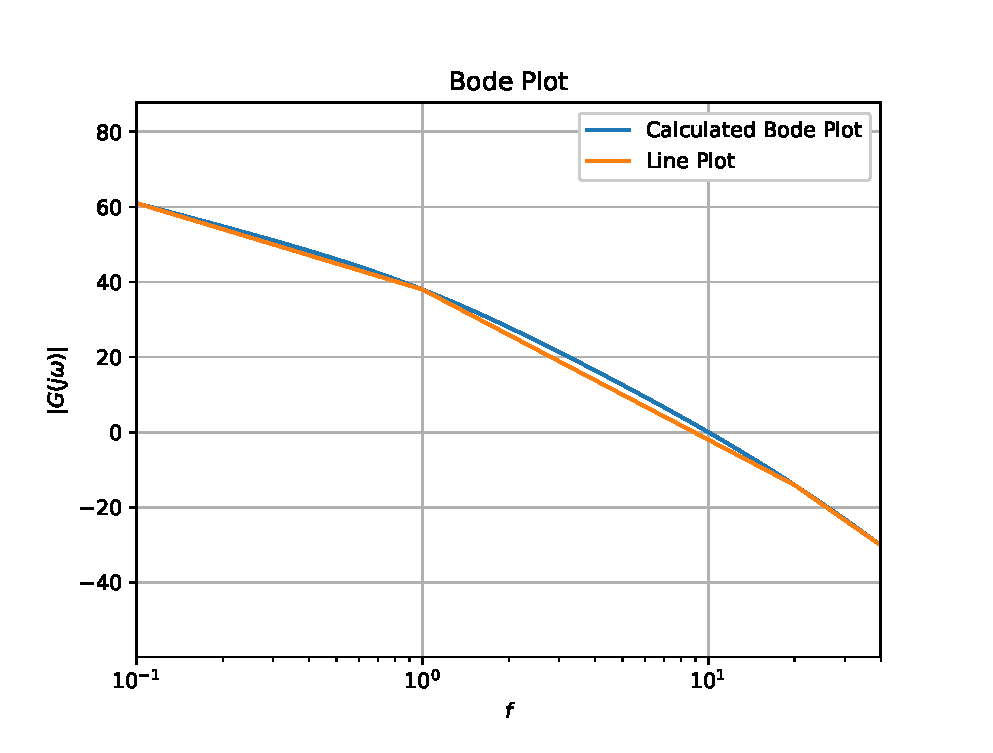
\includegraphics[width= \columnwidth]{./figs/ee18btech11009/ee18btech11009.eps}
	\caption{}
	\label{fig:ee10btech11009_line_plot}
\end{figure} 

\item  Verify if at very high frequency $(\omega \to \infty)$, the phase angle $ \angle G(j\omega)=-3\pi/2$.
\\
\solution
Phase $ \phi $ is the sum of all the phases corresponding to each pole and zero.
%------------------------------------------------
  \begin{align}
 \Rightarrow  G(j\omega) &=  \frac{k}{j\omega(1+j\omega)(20+j\omega)}
\\
\implies  \phi &=  -\tan^{-1}\brak{ {\frac{\omega}{0}}} - \tan^{-1}\brak{\omega} 
\nonumber\\
& \quad - \tan^{-1}\brak{ \frac{\omega}{20}}
\\
 & =  - 90\degree - \tan^{-1}\brak{\omega} - \tan^{-1}\brak{ \frac{\omega}{20}}
\\
\implies  \lim_{\omega \to \infty}   \phi &=    -3\pi/2 
 \end{align} 

 \end{enumerate}
